\documentclass[10,a4paperpaper,]{article}

  \title{End of Session August Report}
  \author{Teaching Lab}
  \date{\today}
  


\newcommand{\logo}{teachinglab_logo.png}
\newcommand{\cover}{cover.png}
\newcommand{\iblue}{04abeb}
\newcommand{\igray}{d4dbde}

% Author: Karol KozioL
% License: GPL-3
% Modified by: Sarah Wagner

% % % packages -----------------------------------------------------------------------------------
\usepackage{amsmath}
\usepackage{array}
\usepackage{booktabs}
\usepackage{calc}
\usepackage{eso-pic}
\usepackage{fancyhdr}
\usepackage{fontspec}
\usepackage[left = 2.5cm, right = 2.5cm, top = 1.2cm, bottom = 1.2cm, includeheadfoot]{geometry}
\usepackage{graphicx}
\usepackage[utf8]{inputenc}
\usepackage{lastpage}
\usepackage{multirow}
\usepackage{tabularx} 
\usepackage{tikz}
\usepackage{titlesec}
\usepackage{xcolor, colortbl}

% % % settings -----------------------------------------------------------------------------------

% % custom colors
\definecolor{iblue}{HTML}{\iblue}
\definecolor{igray}{HTML}{\igray}
% % empty tightlist fix
\def\tightlist{}

% definition of pagename
\newcommand\pagename{Page}

% % fonts 
\defaultfontfeatures{Mapping = tex-text}
\setmainfont[BoldFont = calibri-bold.otf, ItalicFont = calibri-italic.otf, BoldItalicFont = calibri-bold-italic.otf]{calibri.otf}
\newfontfamily\headingfont[ItalicFont = calibri-italic.otf]{calibri.otf}


% % sections
\titleformat{\section}{\color{iblue}\headingfont\Large\bfseries}{\thesection}{1em}{}[\titlerule]
\titleformat{\subsection}{\color{iblue}\headingfont\large\bfseries}{\thesubsection}{1em}{}
\titleformat{\subsubsection}{\color{iblue}\headingfont\bfseries}{\thesubsubsection}{1em}{}

% % misc
\setlength{\parindent}{0em} 
\linespread{1}
\raggedright
\newcolumntype{C}{>{\centering\arraybackslash}X}


% % % custom titlepage ----------------------------------------------------------------------------
\newcommand\BackgroundPic{%
	\put(0,0){%
		\parbox[b][\paperheight]{\paperwidth}{%
			\vfill
			\centering
			
\includegraphics[width=\paperwidth,height=\paperheight]{\cover}%
			\vfill
}}}

\makeatletter

% pagestyle titlepage
\fancypagestyle{customtitle}{
	\lhead{}
	\chead{}
	\rhead{}
	\makeatother
	\lfoot{}
	\cfoot{}
	\rfoot{
\includegraphics{\logo}}
}


% titlepage
\renewcommand{\maketitle}{
	\thispagestyle{customtitle}
	\AddToShipoutPicture*{\BackgroundPic}
	\ClearShipoutPicture
	
	\phantom{a}\hfill
	\vspace{14cm}
	
	\begin{tabular}[l]{@{}p{\textwidth}@{}}
		\color{iblue}\headingfont\LARGE\@title\\[1em]
		\color{iblue}\headingfont\large\@author\\[1em]
		\color{iblue}\headingfont\small\@date\\[1em]
	\end{tabular}
	
	
	
	\clearpage
}
\makeatother

% % % header and footer ---------------------------------------------------------------------------
\pagestyle{fancy}
\lhead{}
\chead{}
\rhead{ 
\includegraphics{\logo}}
\makeatother
\newlength{\myheight}
\lfoot{}
\cfoot{}
\rfoot{\pagename~\thepage \hspace{1pt} / \pageref{LastPage}}
\renewcommand\headrulewidth{0pt}
\renewcommand\footrulewidth{0pt}




\begin{document}


\renewcommand{\contentsname}{Table of Contents}

\renewcommand{\pagename}{Page}


\maketitle
\tableofcontents
\addcontentsline{toc}{section}{Contents}
\clearpage

\section{Likert Ratings}

From August 1 to August 31 there were 64 responses given by San Diego
Unified School District participants, they largely gave positive
feedback when asked questions about a variety of ways to assess the
effectiveness of the facilitation of their courses.

\begin{center}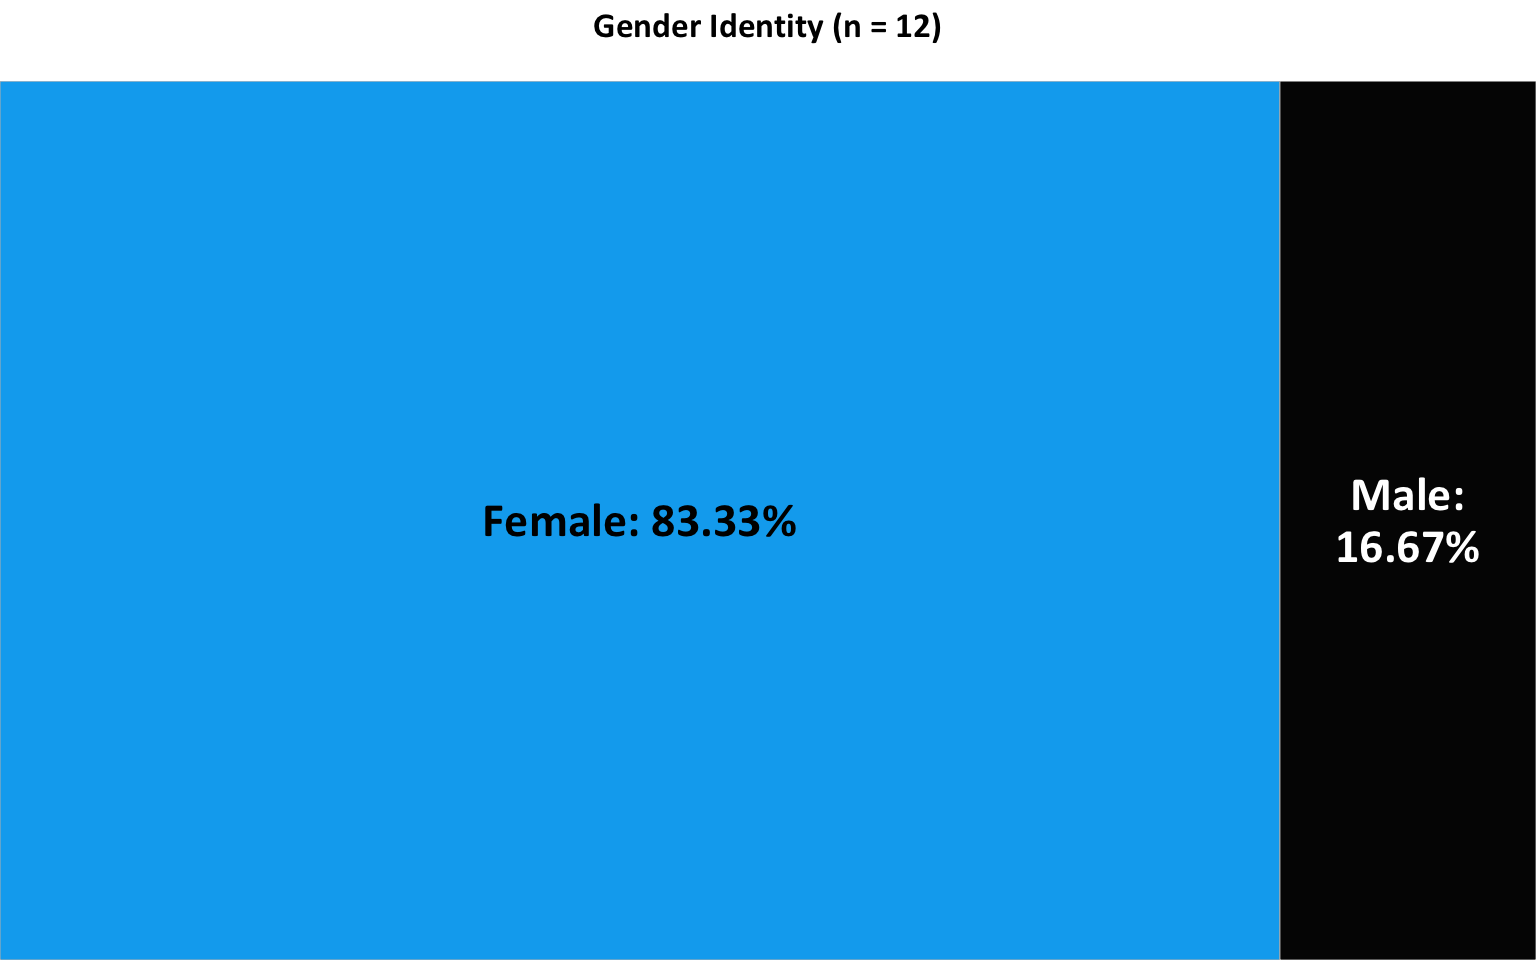
\includegraphics{mathematica_end_of_session_august_files/figure-latex/unnamed-chunk-1-1} \end{center}

\subsection{Percent Agree and Strongly Agree}

In summary, we see the following \% agree or strongly agree with the
above statements:

\begin{itemize}
\tightlist
\item
  79\% strongly agree or agree that they were fully prepared for the
  session.
\item
  67\% strongly agree or agree that they responded to the group's needs.
\item
  76\% strongly agree or agree that they facilitated the content
  clearly.
\item
  76\% strongly agree or agree that they effectively built a safe
  learning community.
\item
  86\% strongly agree or agree that they demonstrated deep knowledge of
  the content they facilitated.
\end{itemize}

\section{Over Time}

In this section responses are illustrated on a daily basis.

\begin{center}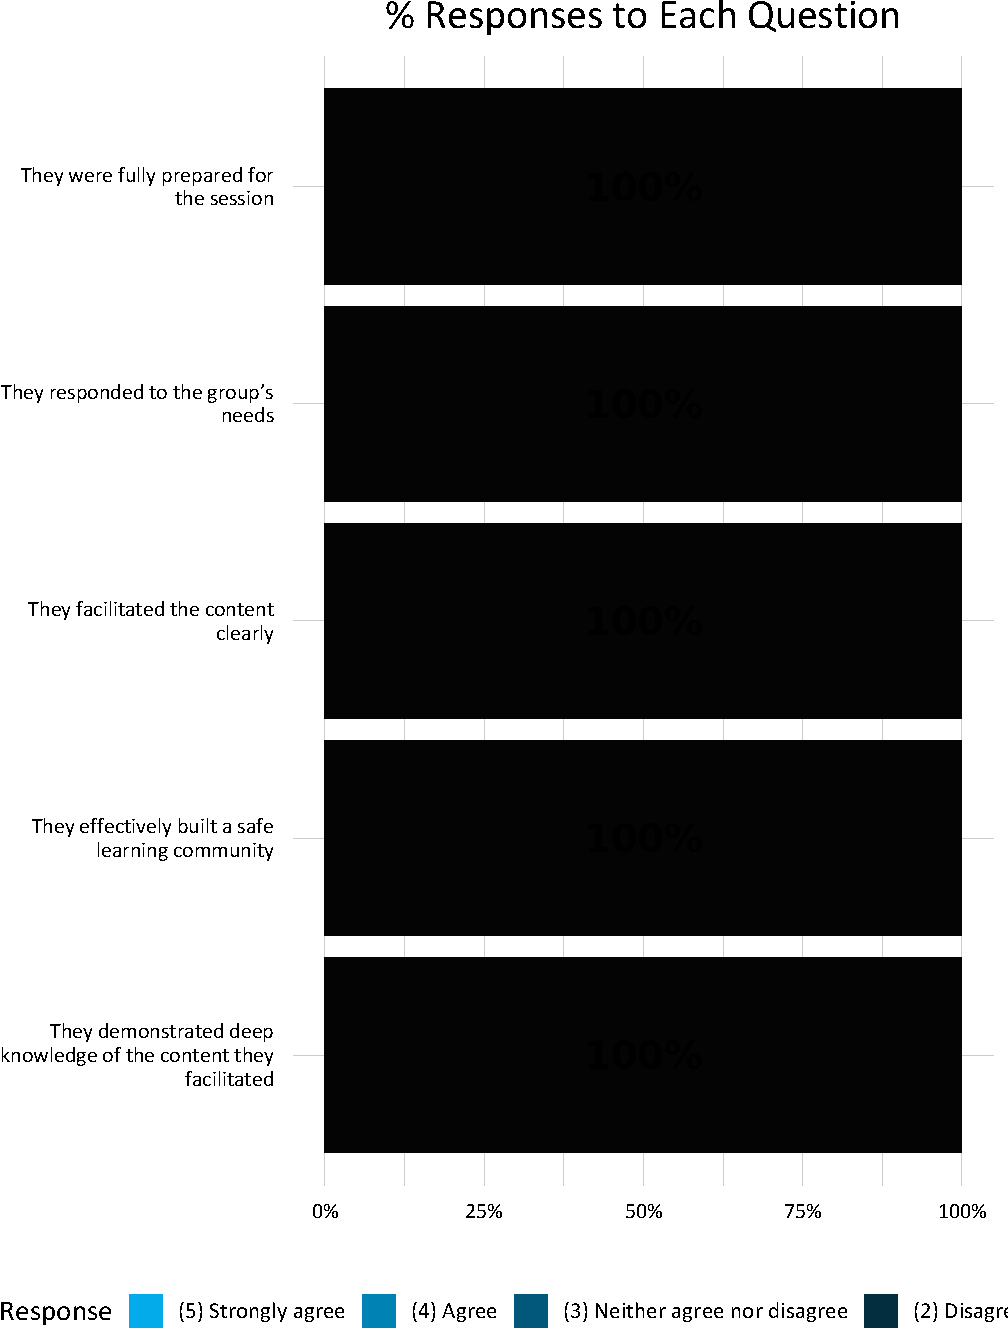
\includegraphics{mathematica_end_of_session_august_files/figure-latex/unnamed-chunk-2-1} \end{center}

\section{Qualitative Participant Feedback}

Finally responses to the following questions are presented below:

\begin{itemize}
\item
  What could have been better about today's session?
\item
  What went well in today's session?
\item
  What additional feedback do you have about their facilitation skills?
\end{itemize}

\subsection{What could have been better about today's session?}

\begin{center}\includegraphics[width=3.07in]{/Users/dunk/Teaching Lab/Coding/TeachingLab/Images/2021-2022/Mathematica/img1} \end{center}

\subsection{What went well in today's session?}

\begin{center}\includegraphics[width=3.67in]{/Users/dunk/Teaching Lab/Coding/TeachingLab/Images/2021-2022/Mathematica/img2} \end{center}

\subsection{What additional feedback do you have about their facilitation skills?}

\begin{center}\includegraphics[width=6.04in]{/Users/dunk/Teaching Lab/Coding/TeachingLab/Images/2021-2022/Mathematica/img3} \end{center}


\end{document}
